\documentclass[10pt,aspectratio=169]{beamer}

\usepackage[utf8]{inputenc}
\usetheme{Berkeley}
\usecolortheme{spruce}

%font
\usepackage{lmodern}% http://ctan.org/pkg/lm

% for degree symbol
\usepackage{textcomp}

% compile only one certain frame
%\includeonlyframes{1}

\usepackage{tikz}
\usetikzlibrary{arrows.meta,shapes.arrows}
%\usetikzlibrary{external}
%\tikzexternalize

\tikzset{
  every overlay node/.style={
    draw=black,fill=white,rounded corners,anchor=north west,
  },
}
% Usage:
% \tikzoverlay at (-1cm,-5cm) {content};
% or
% \tikzoverlay[text width=5cm] at (-1cm,-5cm) {content};
\def\tikzoverlay{%
   \tikz[baseline,overlay]\node[every overlay node]
}%

% for strikethrough
\usepackage{ulem}

\setbeamerfont{section in sidebar}{size=\fontsize{4pt}{4pt}}
\setbeamerfont{subsection in sidebar}{size=\fontsize{4pt}{4pt}}

\graphicspath{{./images/}}

%Information to be included in the title page:
\title{Atmospheric Effects for CMB Ground-Based Observations}
\subtitle{The Case of the LSPE/Strip Telescope}
\author{Matteo Savatteri}
\institute{Università degli Studi di Milano}
\date{\today}

\begin{document}

\frame{\titlepage}

\section*{Outline}
\begin{frame}
\frametitle{Table of Contents}
\tableofcontents
\end{frame}

\section{Introduction}
\subsection{CMB Radiation and B-Modes}

\begin{frame}
\frametitle{CMB Radiation}

\begin{itemize}
\item $\sim$380000 after Big Bang $\rightarrow$ $\sim$3000 K $\rightarrow$ recombination $\rightarrow$
      black body radiation \pause
\item Universe expansion $\rightarrow$ 2.7255 K \pause
\item $T$ anisotropies $\rightarrow$ signature primordial perturbations \pause
\end{itemize}

\vspace{15pt}

Thomson Scattering $T$ anisotropies $\rightarrow$ CMB Polarization: \pause
\begin{itemize}
\item E-modes $\rightarrow$ even parity \pause
\item B-modes $\rightarrow$ odd parity
\end{itemize}

\pause

\begin{tikzpicture}[remember picture,overlay]
\node at (6,2) {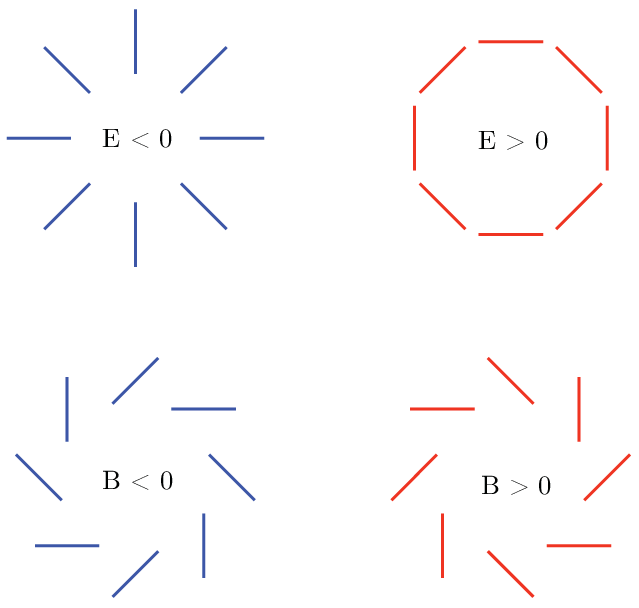
\includegraphics[width=0.5\textwidth]{E-mode-and-B-mode}};
\end{tikzpicture}

\end{frame}

\begin{frame}
\frametitle{PGW B-modes}

\begin{itemize}
\item<1-> high $l$ $\rightarrow$ gravitational lensing E-modes\pause
\item<2-> low $l$ $\rightarrow$ \alert{primordial gravitational waves}:
\begin{itemize}
\item<4-> Correlation pattern\\ $\rightarrow$ $\frac{\Delta T}{T} \leq 10^{-6}$
\end{itemize}

\pause

\onslide<3->{%
\tikz\node at (4.5,-0.8) [fill=blue,shape=single arrow,text width=3.6cm,text height=2.5ex,rotate=-90,overlay] {};

\vspace{80pt}
\centering
\LARGE
\alert{\textit{Smoking gun} inflactionary paradigm}
}

\end{itemize}

\end{frame}

\subsection{LSPE/Strip}

\begin{frame}[label=1]
\frametitle{LSPE/Strip}

\begin{columns}
\column{0.4\textwidth}

\begin{itemize}
\item<1-> Observation microwave sky at large angular scale
\item<2-> Detection of B-modes
\item<3-> \only<3>{Balloon-borne}\only<4->{\sout{Balloon-borne}}
          \onslide<4->{$\rightarrow$ ground based: Observatorio del Teide, Tenerife}
\item<5-> Focal plane:

\begin{itemize}
\item<5-> 49 detectors \onslide<6->{$\rightarrow$\\ coherent polarimeters}
          \onslide<7->{$\rightarrow$\\ 43 GHz (Q-band)}
\item<8-> 6 detectors $\rightarrow$\\ 95 GHz (W-band)
\end{itemize}

\end{itemize}

\column{0.6\textwidth}
\centering
\includegraphics<4>[height=0.94\textheight]{strip-telescope}
\includegraphics<5->[width=1\textwidth]{strip-focal-plane}
\end{columns}

\end{frame}

\section{Atmospheric Emission Model}
\subsection{Equation of Atmospheric Radiative Transfer}

\begin{frame}
\frametitle{Atmospheric Radiative Balance}

\begin{itemize}
\item<1-> Atmosphere $\rightarrow$ \alert{dispersive} medium $\rightarrow \epsilon = \epsilon_R + i\epsilon_I$
\item<2-> \only<2-3>{$\epsilon_R \propto \sqrt{n_\nu}$}\only<4->{\sout{$\epsilon_R \propto \sqrt{n_\nu}$}},
          \quad $\epsilon_I \propto \alpha_\nu$ \onslide<3->{$\rightarrow$  $O_2$, $H_2O$}
\end{itemize}


\begin{block}{Radiative Transfer Equation}<5->
\begin{equation}
\frac{dI_\nu}{ds} = -\alpha I_\nu + j_\nu
\end{equation}
\end{block}

\begin{block}{Kirchhoff Law \onslide<7->{\textcolor{red}{(Valid for system at LTE e.g ELA)}}}<6->
\begin{equation}
B_\nu(T) = \frac{j_\nu(T)}{\alpha_\nu(T)}
\end{equation}
\end{block}

\end{frame}

\subsection{Atmospheric Brightness Temperature}

\begin{frame}
\frametitle{Atmospheric Brightness Temperature}

Solution radiative transfer equation $\rightarrow$ KL $\rightarrow$ $j_\nu = \alpha_\nu B_\nu(T_{atm}^{ph})$ :

\onslide<2->{
\begin{equation}
\frac{1}{\alpha_\nu}\frac{dI_\nu}{ds} = -\frac{dI_\nu}{d\tau} = -I_\nu + B_\nu\left(T_{atm}^{ph}\right)
\end{equation}
}

\onslide<3->{Integrating from ground to \alert{tropopause} and applaying RJ approximation:}

\begin{block}{Atmospheric Brightness Temperature}<4->
\only<1-5>{%
\begin{equation}
T_{sky}(\nu) = \textcolor<5>{red}{T_{atm}^{ph}(1 - e^{-\tau_A(\nu)})} + T_{CMB}(\nu)e^{-\tau_A(\nu)}
\end{equation}
}%
\only<6->{%
\begin{equation}
\textcolor{red}{T_{atm}^A(\nu)} = T_{sky}(\nu) - T_{CMB}(\nu)e^{-\tau_A(\nu)}
\end{equation}
}%
\end{block}

\onslide<7->{Computational approach:}
\begin{itemize}
\item<7-> Atmosphere discretization into \alert{layers}
\item<8-> Write radiative transfer equation for each layer \onslide<10->{$\rightarrow$ \textcolor{red}{input?}}
\item<9-> Solve this system of equations
\end{itemize}

\end{frame}

\section{Atmospheric Statistical Picture}

\subsection{ECMWF ERA5 Atmospheric Reanalisys}

\begin{frame}
\frametitle{ECMWF ERA5 Atmospheric Reanalisys}

\begin{itemize}
\item<1-8> Estimates large number of climate variables
\item<2-8> Earth covered
\item<3-8> $\sim$40 years of data (1980-2020)
\item<4-8> Spatial resolution $\rightarrow$ 0.25\textdegree ($\sim$30 Km)
\item<5-8> Temporal resolution $\rightarrow$ 1 hour
\end{itemize}

\onslide<6-8>{
\tikz\node at (6.5,-0.2) [fill=blue,shape=single arrow,text width=2.5cm,text height=2.5ex,rotate=-25,overlay] {};

\vspace{1.3cm}
\large
\hspace{5.2cm}\alert{Good spatial and temporal resolution!}
}

\only<7>{
\begin{tikzpicture}[remember picture,overlay]
\node at (6,2.5) {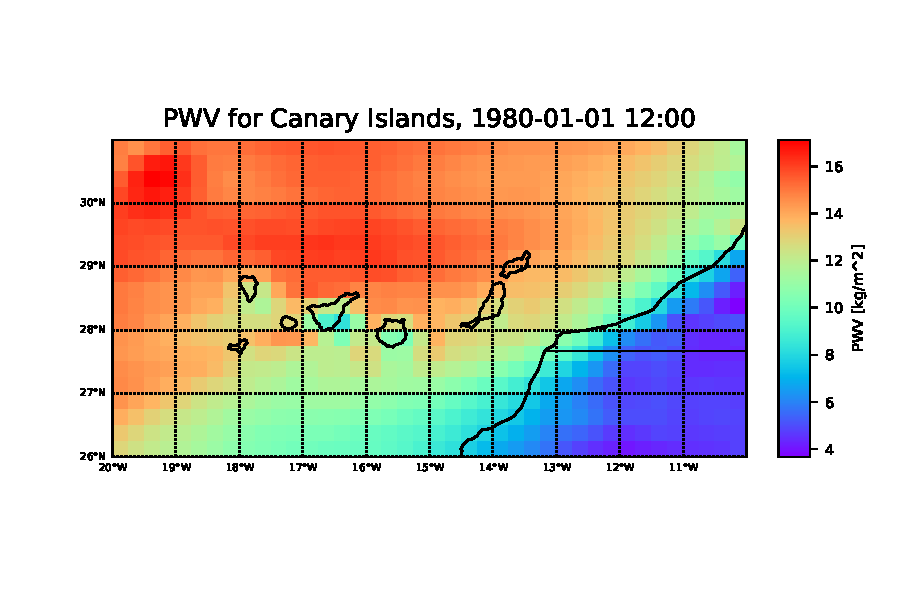
\includegraphics[width=1.15\textwidth]{PWV_Canary_Islands_1980-01-01_12-00}};
\end{tikzpicture}
}

\only<8>{
\vspace{0.2cm}
\hspace{7cm}\textcolor{red}{\textbf{But not enough}}
}

\only<9>{
\begin{tikzpicture}[remember picture,overlay]
\node at (6,2.5) {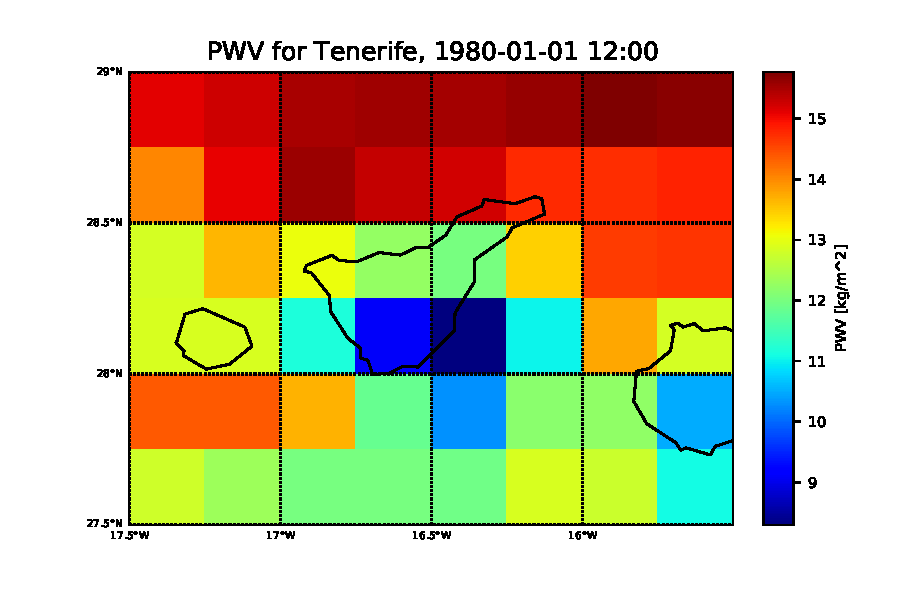
\includegraphics[width=0.9\textwidth]{PWV_Tenerife_1980-01-01_12-00}};
\end{tikzpicture}
}

\end{frame}

\subsection{CDFs \texttt{.fits} File}

\begin{frame}
\frametitle{CDFs \texttt{.fits} File}

\begin{columns}
\column{0.3\textwidth}

\onslide<1-15>{Statistical picture:}
\small
\begin{itemize}
\item<2-15> Set of \alert{\textit{CDFs}} for every
          hour, month, \alert{relevant parameter}
\item<5-15> $\sim$2MB \texttt{.fits} file
\item<15-15> \alert{Seasonal matrices}
\end{itemize}%

\column{0.7\textwidth}
\only<3-5>{
\tikz\node at (1.7,-2) [fill=blue,shape=single arrow,text width=3cm,text height=2.5ex,overlay] {};

\begin{itemize}
\addtolength{\itemindent}{4cm}
\item TQL
\item TQI
\item \textcolor<4-5>{red}{TQV}
\item \textcolor<4-5>{red}{TS}
\item \textcolor<4-5>{red}{PS}
\item T10M
\item V10M
\item U10M
\end{itemize}
}
%
% Avoid spacing issue with images '%'
\includegraphics<6>[width=1.2\textheight]{PWV_Monthly_CDFs/PWV_Monthly_CDFs_Hour_0}%
\includegraphics<7>[width=1.2\textheight]{PWV_Monthly_CDFs/PWV_Monthly_CDFs_Hour_2}%
\includegraphics<8>[width=1.2\textheight]{PWV_Monthly_CDFs/PWV_Monthly_CDFs_Hour_5}%
\includegraphics<9>[width=1.2\textheight]{PWV_Monthly_CDFs/PWV_Monthly_CDFs_Hour_8}%
\includegraphics<10>[width=1.2\textheight]{PWV_Monthly_CDFs/PWV_Monthly_CDFs_Hour_11}%
\includegraphics<11>[width=1.2\textheight]{PWV_Monthly_CDFs/PWV_Monthly_CDFs_Hour_14}%
\includegraphics<12>[width=1.2\textheight]{PWV_Monthly_CDFs/PWV_Monthly_CDFs_Hour_17}%
\includegraphics<13>[width=1.2\textheight]{PWV_Monthly_CDFs/PWV_Monthly_CDFs_Hour_20}%
\includegraphics<14>[width=1.2\textheight]{PWV_Monthly_CDFs/PWV_Monthly_CDFs_Hour_23}%
\includegraphics<15>[width=1.2\textheight]{Median_PWV_Matrix}

\only<16>{
\begin{tikzpicture}[remember picture,overlay]
\node at (2.6,-0.25) {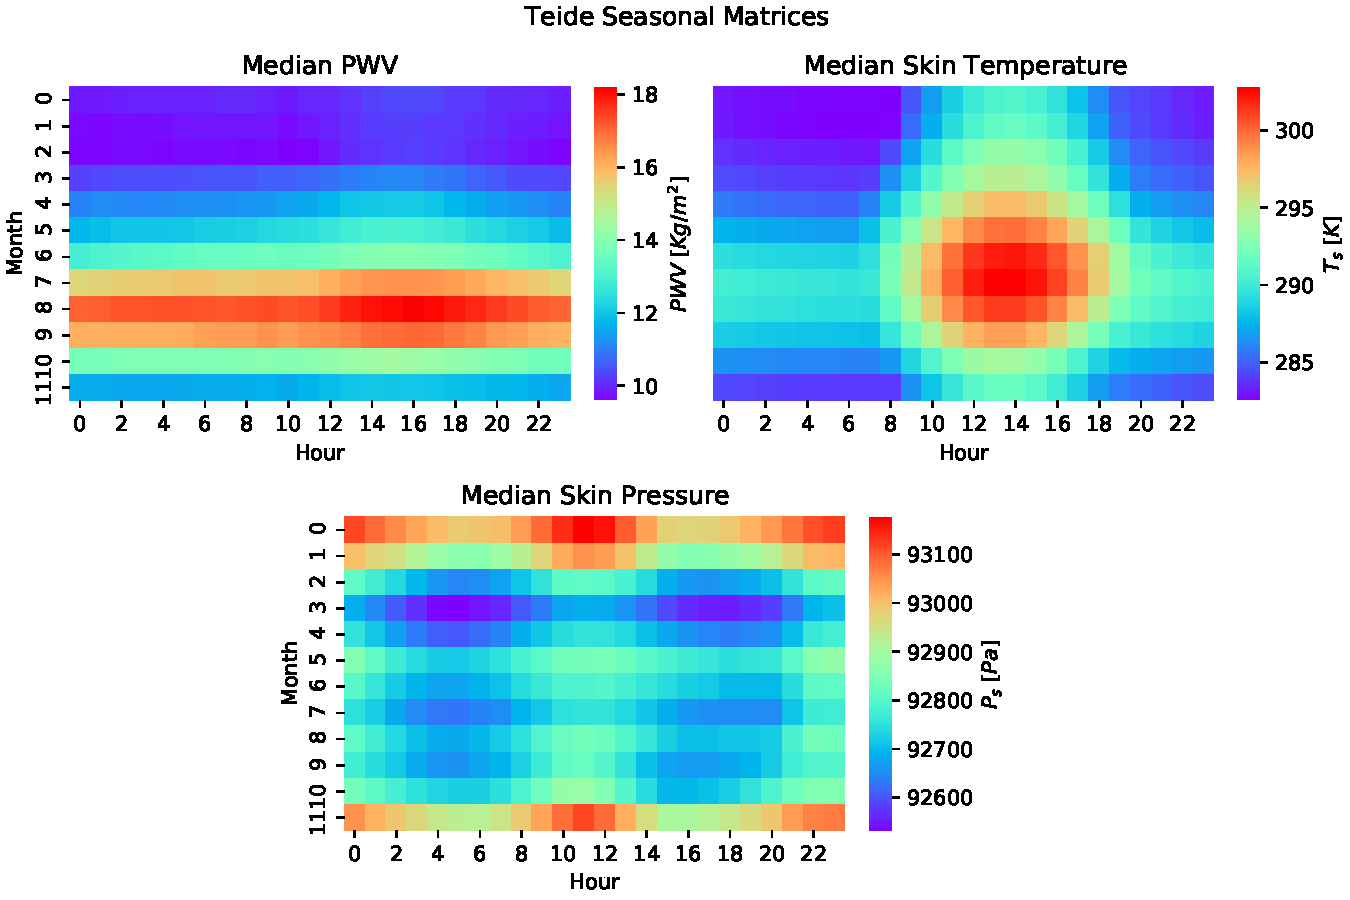
\includegraphics[width=1.18\textwidth]{Teide_Seasonal_Matrices}};
\end{tikzpicture}
}

\end{columns}

\end{frame}

\subsection{CMB Atmospheric Library}

\begin{frame}
\frametitle{CMB Atmospheric Library (\texttt{CAL})}

\begin{itemize}
\item<1-> \texttt{C++} core with \alert{\texttt{Python} bindings}
\item<2-> Atmospheric simulation code from \alert{\texttt{TOAST} framework} $\rightarrow$ CMB ground based telescopes
\item<3-> \alert{Open source} code on Github $\rightarrow$ \textcolor{blue}{\url{https://github.com/cmbgroundbased/cal}}
\item<4-> Realizations of meteorological parameters with Monte Carlo method
\end{itemize}

\vspace{0.5cm}
\onslide<5->{Relevant methods:}

\vskip0pt plus 1filll

\only<6>{
\begin{block}{\texttt{Weather}}
Input $\rightarrow$ CDFs \texttt{.fits}, Time\\
Output $\rightarrow$ realizations of meteorological parameters from
                     the atmospheric statistical picture
\end{block}
}

\only<7>{
\begin{block}{\texttt{atm\_atmopheric\_loading}}
Wrapper around \texttt{libaatm} methods $\rightarrow$ solves equation of radiative transfer
$\rightarrow$ discretisation of the atmosphere predefined series of layers\\
Input $\rightarrow$ $T_s$, $P_s$, PWV, $\nu$\\
Output $\rightarrow$ $T_{sky}(\nu)$
\end{block}
}

\only<8>{
\begin{block}{\texttt{atm\_absorption\_coefficient}}
Wrapper around \texttt{libaatm} methods\\
Input $\rightarrow$ $T_s$, $P_s$, PWV, $\nu$\\
Output $\rightarrow$ $1 - e^{-\tau_A(\nu)}$
\end{block}
}

\vspace{1cm}

\end{frame}

\section{Comparison with Measurements}
\subsection{Raw Simulation-QUIJOTE Data Comparison}

\begin{frame}
\frametitle{QUIJOTE-MFI Dataset}

\only<1-10>{
QUIJOTE QT1 Telescope:
\begin{itemize}
\item<2-> \alert{Teide} Observatory
\item<4-> Instituto de Astrofisica de Canarias
\item<5-> \alert{MFI} (Multi Frequency Instrument) \onslide<6->{$\rightarrow$ Central frequencies
          \alert{11}, \alert{13}, \alert{17}, \alert{19} GHz}
\item<7-> $T_{atm}$ data from MFI \textit{sky dips}:

\begin{itemize}
\item<8-> \alert{444} points $\rightarrow$ December 2012-February 2015
\item<9-> \alert{32} Channels
\item<10-> \alert{Inhomogeneous time} distribution
\end{itemize}

\end{itemize}
}

\only<3>{
\begin{tikzpicture}[remember picture,overlay]
\node at (6.5,2) {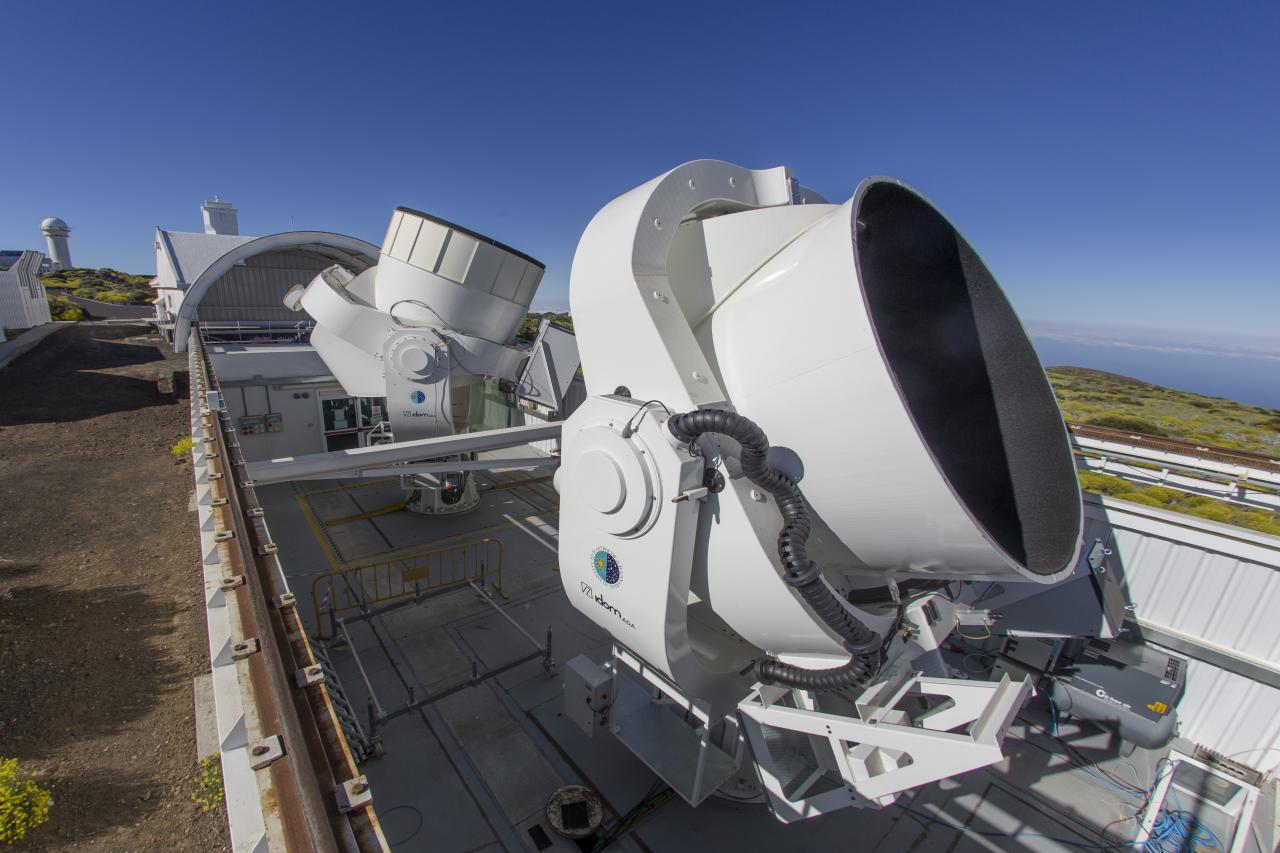
\includegraphics[width=0.75\textwidth]{QUIJOTE}};
\end{tikzpicture}
}

\only<11->{
\begin{tikzpicture}[remember picture,overlay]
\node at (6.6,-0.4) {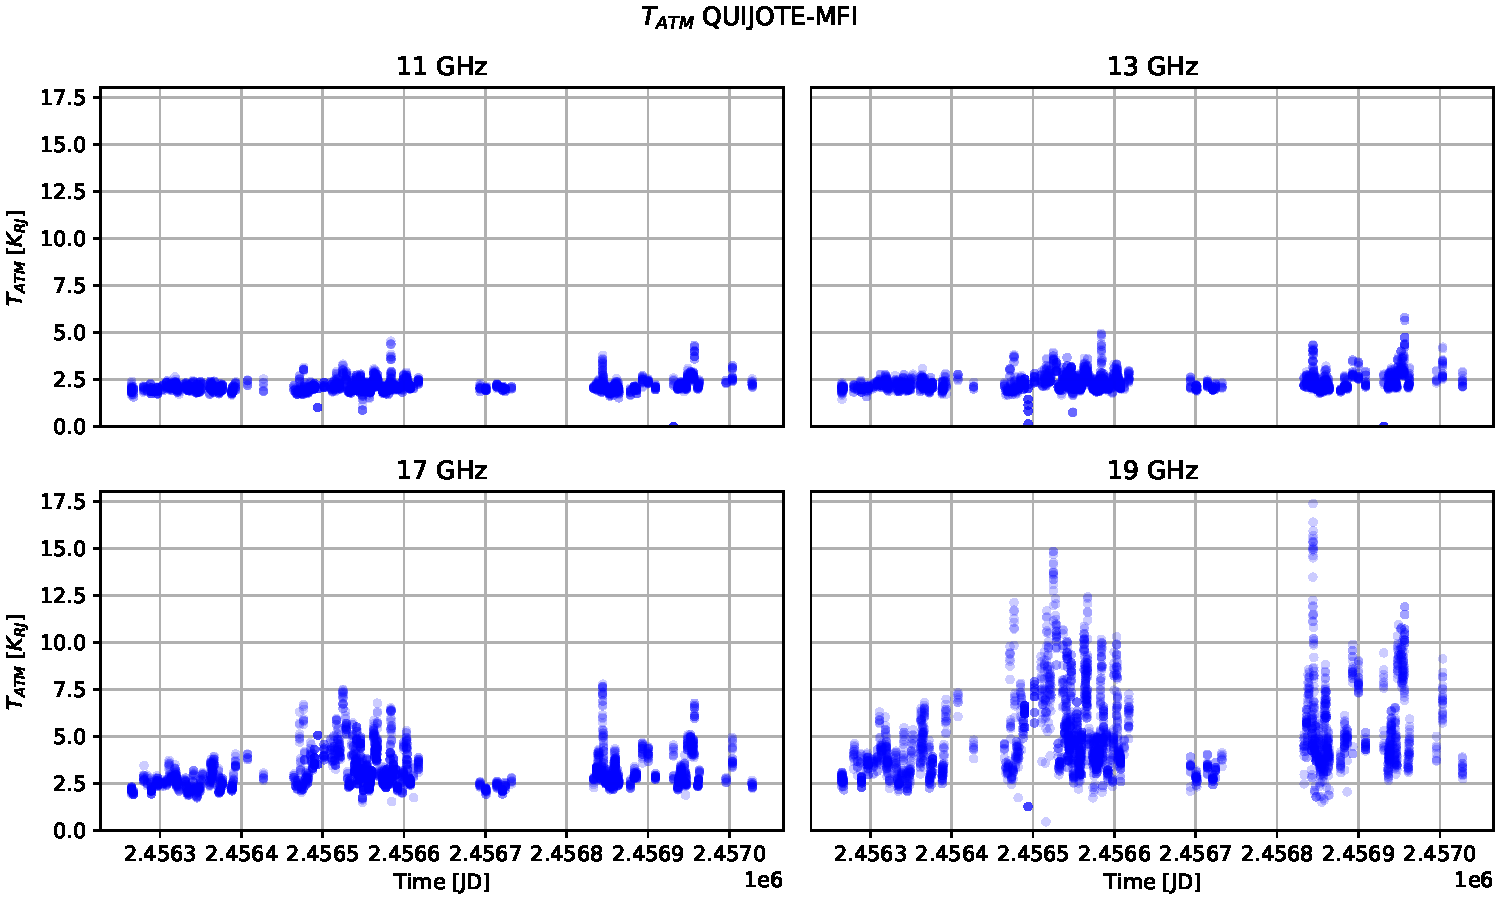
\includegraphics[width=0.87\textwidth]{QUIJOTE_Dataset}};
\end{tikzpicture}
}
%
%\only<12-14>{
%\tikzoverlay[text width=8cm] at (2.5,1) {
%\begin{block}{Atmospheric Brightness Temperature}
%\begin{equation}
%\textcolor<13>{red}{T_{sky}(\nu)} = \textcolor<14>{red}{T_{atm}^{ph}(1 - e^{-\tau_A(\nu)})} + T_{CMB}(\nu)e^{-\tau_A(\nu)}
%\end{equation}
%\end{block}
%};
%}

\end{frame}

\begin{frame}
\frametitle{Comparison with QUIJOTE Data}

\centering
\includegraphics<1>[height=0.9\textheight]{QUIJOTE-Sim_raw/QUIJOTE_Sim_Comparison_no_cal_11GHz}%
\includegraphics<2>[height=0.9\textheight]{QUIJOTE-Sim_raw/QUIJOTE_Sim_Comparison_no_cal_13GHz}%
\includegraphics<3>[height=0.9\textheight]{QUIJOTE-Sim_raw/QUIJOTE_Sim_Comparison_no_cal_17GHz}%
\includegraphics<4->[height=0.9\textheight]{QUIJOTE-Sim_raw/QUIJOTE_Sim_Comparison_no_cal_19GHz}%
%
\only<5->{%
\tikzoverlay[text width=8cm] at (-8.9,4.3) {
\begin{itemize}
\item<5-> Simulation overestimates data
\item<6-> Overestimation gets worse for higher frequencies
\end{itemize}
};
}%

\end{frame}

\subsection{Calibrated Simulation-QUIJOTE Data Comparison}

\begin{frame}
\frametitle{Teide Pixel}

\centering
\includegraphics<1>[height=\textheight]{PWV_Tenerife_1980-01-01_12-00}%
\includegraphics<2->[height=0.92\textheight]{PWV_Teide_1980-01-01_12-00}%
%
\only<3->{%
\tikz\draw[red,fill=red,overlay,remember picture] (-7.3,5.4) circle (1ex);%
}%
\only<4->{%
\tikz\node[yellow,overlay,remember picture,rotate=45] at (-6.8,3.8) {Low lands};%
}%
\only<5->{%
\tikz\node[yellow,overlay,remember picture] at (-4.5,2.3) {Ocean};%
}%

\end{frame}

\begin{frame}
\frametitle{Calibration Coefficient}

\onslide<1-7,11-12,15>{\alert{\texttt{AM}} $\rightarrow$ Computer program for radiative transfer computations}
\begin{itemize}
\item<2-7,11-12,15> Input $\rightarrow$ \alert{User defined} atmospheric profile, $\nu$ range and step
\item<3-7,11-12,15> Output $\rightarrow$ $T_{sky}(\nu)$, $\tau_A(\nu)$
\end{itemize}

\vspace{1.5cm}

\onslide<4-7,11-12,15>{
\tikz\node at (5.6,1.2) [fill=blue,shape=single arrow,text width=2cm,text height=1ex,rotate=-90,overlay] {};
}

\onslide<4-7,11-12,15>{\alert{Balloon probe measurements} performed at Teide observatory:}
\begin{itemize}
\item<5-7,11-12,15> \alert{High spatial} resolution
\item<6-7,11-12,15> \alert{Low temporal} resolution $\rightarrow$ flight duration $\sim$ 12 hours
\item<7,11-12,15> \alert{One year} of data (2018)
\end{itemize}

%
\only<8>{%
\begin{tikzpicture}[remember picture,overlay]
\node at (6.9,3) {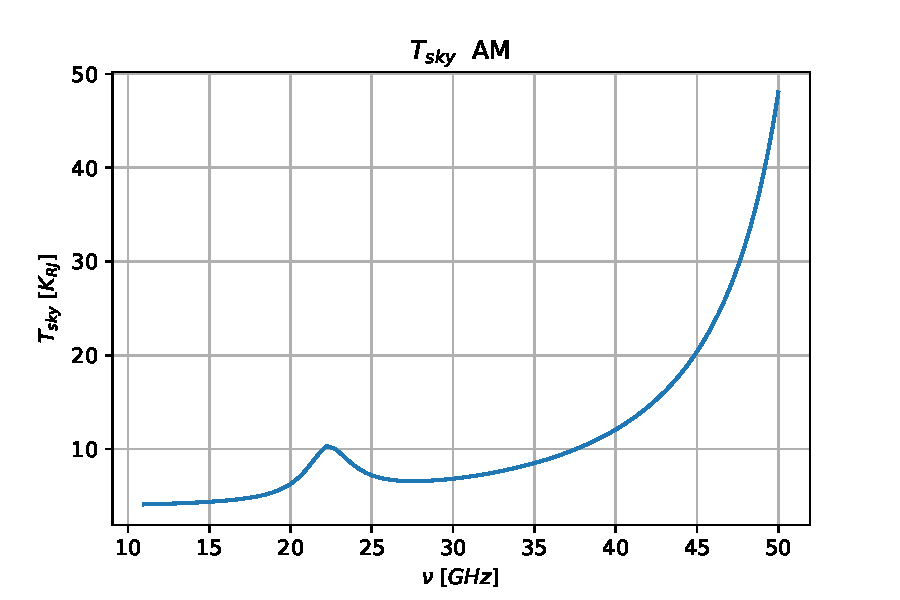
\includegraphics[height=0.92\textheight]{AM}};
\end{tikzpicture}
}%
%
\only<9>{%
\begin{tikzpicture}[remember picture,overlay]
\node at (6.7,2.9) {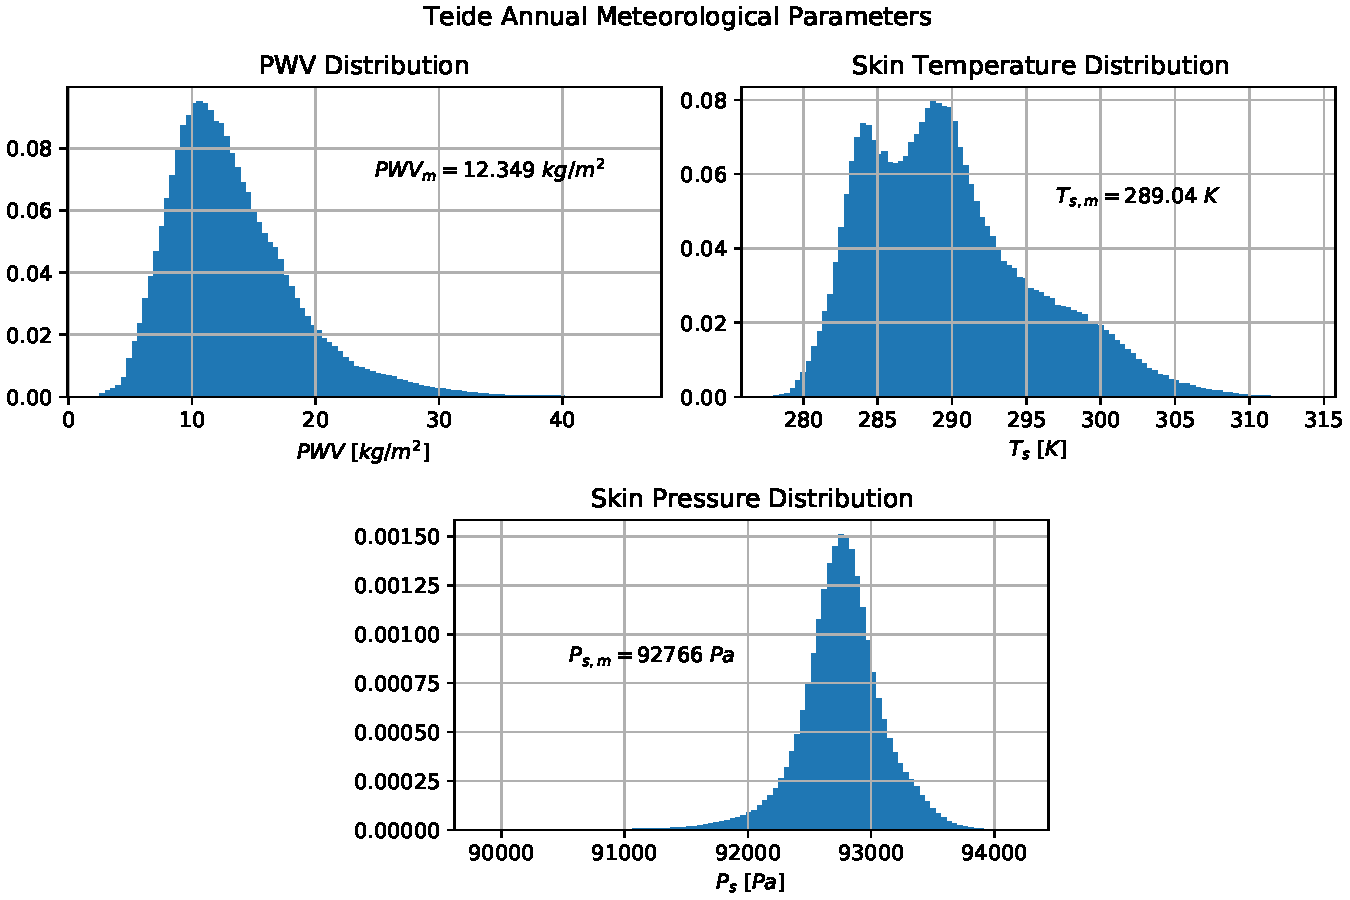
\includegraphics[height=1\textheight]{Teide_Annual_Distributions}};
\end{tikzpicture}
}%
%
\only<10>{%
\begin{tikzpicture}[remember picture,overlay]
\node at (6.9,3) {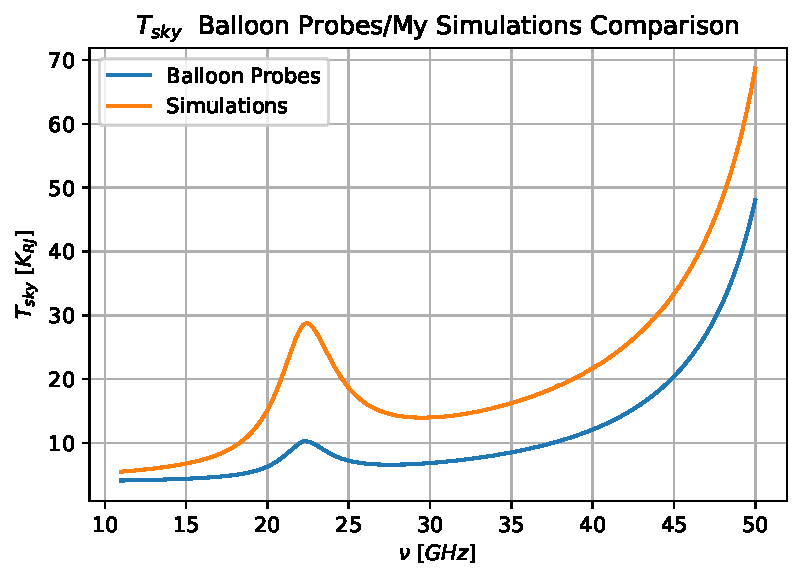
\includegraphics[height=0.92\textheight]{AM_CAL_Comparison}};
\end{tikzpicture}
}%
%
\only<11-12>{%
\tikzoverlay[text width=8cm] at (2.8,4.5) {
\begin{block}{Calibration Coefficient}
\begin{equation}
k(\nu) = \frac{T_{sky}^{AM}(\nu)}{T_{sky}^{CAL}(\nu)}
\end{equation}
\onslide<12>{Assumption: \textcolor{red}{not time dependent!}}
\end{block}
};
}%
%
\only<13>{%
\begin{tikzpicture}[remember picture,overlay]
\node at (6.9,3) {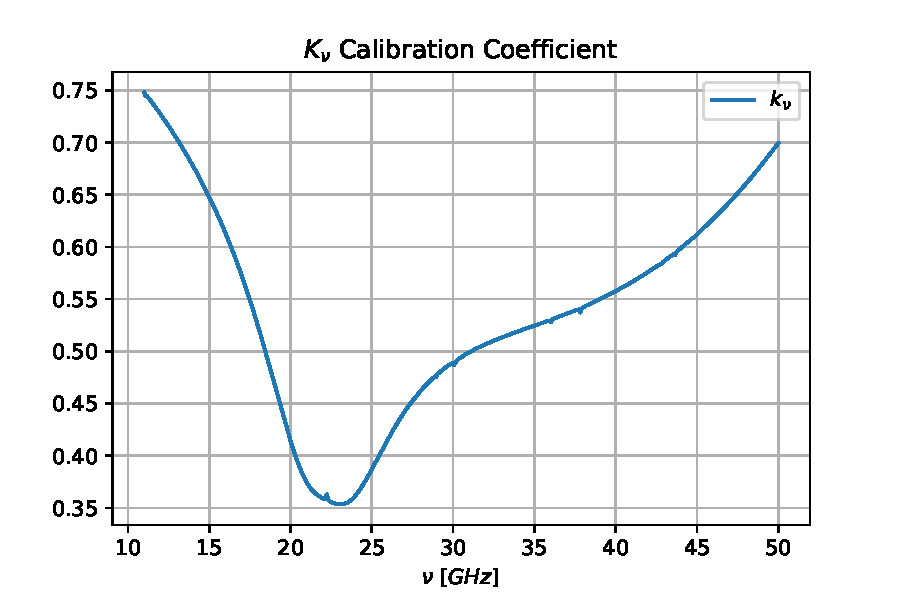
\includegraphics[height=0.92\textheight]{Calibration_Coefficient}};
\end{tikzpicture}
}%
%
\only<14>{%
\begin{tikzpicture}[remember picture,overlay]
\node at (6.9,3) {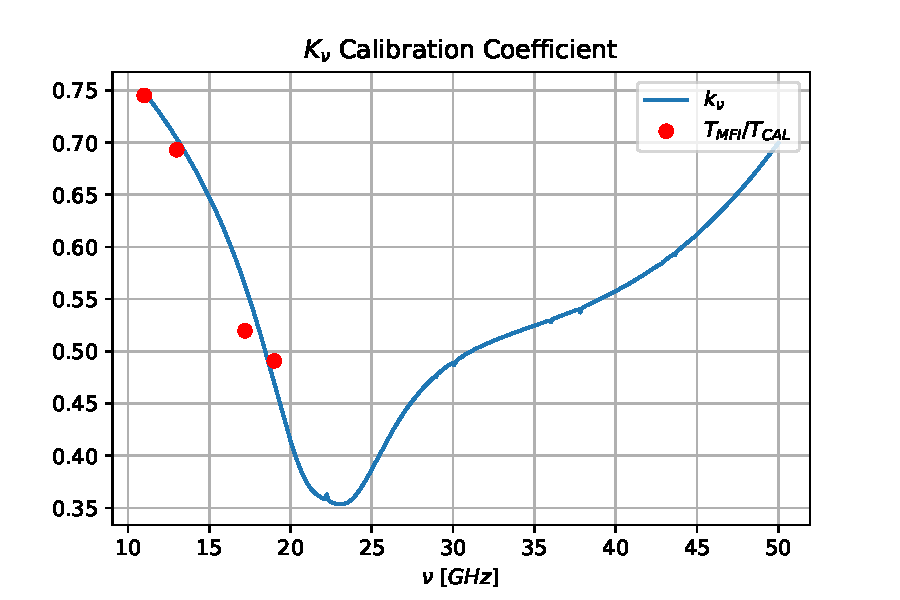
\includegraphics[height=0.92\textheight]{Calibration_Coefficient_QUIJOTE}};
\end{tikzpicture}
}%
%
\only<15>{%
\tikzoverlay[text width=8cm] at (2.8,4.5) {
\begin{block}{Atmospheric Brightness Temperature (Calibrated)}
\begin{equation}
T_{atm}^A(\nu) = k(\nu)[T_{sky}(\nu) - T_{CMB}(\nu)e^{-\tau_A(\nu)}]
\end{equation}
\end{block}
};
}%
%
\end{frame}

\begin{frame}
\frametitle{Comparison with QUIJOTE Data: Calibrated Simulations}

\centering
\includegraphics<1>[height=0.9\textheight]{QUIJOTE-Sim_cal/QUIJOTE_Sim_Comparison_11GHz}%
\includegraphics<2>[height=0.9\textheight]{QUIJOTE-Sim_cal/QUIJOTE_Sim_Comparison_13GHz}%
\includegraphics<3>[height=0.9\textheight]{QUIJOTE-Sim_cal/QUIJOTE_Sim_Comparison_17GHz}%
\includegraphics<4>[height=0.9\textheight]{QUIJOTE-Sim_cal/QUIJOTE_Sim_Comparison_19GHz}

\end{frame}

\subsection{\texttt{tatmget}}

\begin{frame}
\frametitle{\texttt{tatmget}}

\onslide<1->{
\texttt{Python 3} script to simulate statistical populations of seasonal
$T_{atm}$ matrices (Open source and GNU GPLv3 licensed when accomplished)
}

\vspace{0.2cm}

\onslide<2->{Overview:}
\begin{itemize}
\item<2-> Calls \texttt{CAL} methods to simulate $T_{sky}$s
\item<3-> Parallel execution with \texttt{OpenMPI}
\item<4-> Input $\rightarrow$ CDFs \texttt{.fits} file for desired site, $\nu$
\item<5-> \texttt{.npz} cointaning the populations
\end{itemize}

\vspace{0.2cm}

\onslide<6->{Improvements:}
\begin{itemize}
\item<6-> Output populations of meteorological parameters only
\item<7-> Output uncalibrated or calibrated $T_{atm}$s
\item<8-> Output approximated $T_{atm}$s estimating $T_{atm}^{ph}$
\item<9-> Output $T_{atm}$s \alert{convoluted} with \alert{arbitrary bandshapes}\\
\onslide<10->{$\rightarrow$ execution time reduced by a $\sim$ 15 factor from first version}

\end{itemize}

\end{frame}

\section{Bandshape Integration: a Discussion}

\begin{frame}
\frametitle{Strip Q-Band Bandshapes}

\centering
\includegraphics<1>[height=0.92\textheight]{Strip_Bandshapes}%
\includegraphics<2>[height=0.92\textheight]{Strip_Bandshapes+TATM.pdf}%

\end{frame}

\begin{frame}
\frametitle{Bandshape Integration: a Discussion}

\centering
\includegraphics<1>[height=0.98\textheight]{Conluted_TATM_Teide/Convoluted_TATM_Teide_Month_1}%
\includegraphics<2>[height=0.98\textheight]{Conluted_TATM_Teide/Convoluted_TATM_Teide_Month_2}%
\includegraphics<3>[height=0.98\textheight]{Conluted_TATM_Teide/Convoluted_TATM_Teide_Month_3}%
\includegraphics<4>[height=0.98\textheight]{Conluted_TATM_Teide/Convoluted_TATM_Teide_Month_4}%
\includegraphics<5>[height=0.98\textheight]{Conluted_TATM_Teide/Convoluted_TATM_Teide_Month_5}%
\includegraphics<6>[height=0.98\textheight]{Conluted_TATM_Teide/Convoluted_TATM_Teide_Month_6}%
\includegraphics<7>[height=0.98\textheight]{Conluted_TATM_Teide/Convoluted_TATM_Teide_Month_7}%
\includegraphics<8>[height=0.98\textheight]{Conluted_TATM_Teide/Convoluted_TATM_Teide_Month_8}%
\includegraphics<9>[height=0.98\textheight]{Conluted_TATM_Teide/Convoluted_TATM_Teide_Month_9}%
\includegraphics<10>[height=0.98\textheight]{Conluted_TATM_Teide/Convoluted_TATM_Teide_Month_10}%
\includegraphics<11>[height=0.98\textheight]{Conluted_TATM_Teide/Convoluted_TATM_Teide_Month_11}%
\includegraphics<12>[height=0.98\textheight]{Conluted_TATM_Teide/Convoluted_TATM_Teide_Month_12}%

\end{frame}

\begin{frame}
\frametitle{Bandshape Integration: Some Ideas}

\only<1->{Some ideas:}
\begin{itemize}
\item<2-> Atmospheric emission is  unpolarized
\item<3-> Atmospheric signal boosts the white noise
\item<4-> Leakage of $I$ into $Q$ and $U$
\end{itemize}

\end{frame}

\end{document}
